%%%%%%%%%%%%%%%%%%%%%%%%
% $Autor: MansourAhmadyPhoulady, RanjeetsingTawar, HemanthPrabhakaran$
% $Pfad: Car_Licence_Plate_Identification_with_a_JetsonNano$
% $Version: 4.0.0 $
%
% !TeX encoding = utf8
%
%%%%%%%%%%%%%%%%%%%%%%%%

\chapter{Hardware Description}

\section{Introduction to Nvidia Jetson Nano}
The NVIDIA® Jetson Nano™ Developer Kit is a cost-effective, compact AI computing platform designed for makers, learners, and developers. It brings the advanced capabilities of modern artificial intelligence into the hands of a wide range of users through a low-power, user-friendly interface. This platform supports rapid development and prototyping, thanks to its compatibility with a broad spectrum of peripherals, add-ons, and pre-configured projects.

The \textbf{NVIDIA\textsuperscript{\textregistered} Jetson Nano} stands out by leveraging the powerful  \textbf{NVIDIA\textsuperscript{\textregistered} JetPack\textsuperscript{\texttrademark} SDK}, which provides the tools and resources required to execute cutting-edge AI and machine learning workloads seamlessly. The JetPack SDK equips developers with:

\begin{enumerate}
	\item A full-featured desktop Linux OS integrated with NVIDIA drivers
	\item Advanced AI and computer vision libraries and APIs to enable robust AI processing and data analysis
	\item Comprehensive developer tools for coding, debugging, and optimizing applications
	\item Documentation and sample code for quicker learning and efficient development
\end{enumerate}



\section{Hardware Requirements}
\begin{figure}[h!]
	\centering
	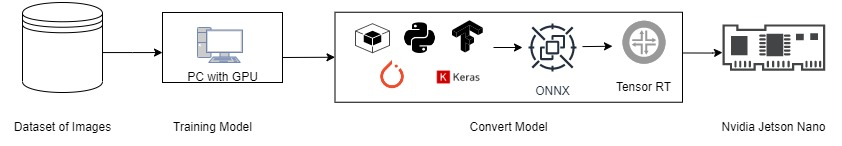
\includegraphics[width=\textwidth]{Images/Hardware-planning}
	\caption{Development and Deployment Process Flow}
\end{figure}
\textbf{Contents of the Developer Kit Box}\\
The NVIDIA Jetson Nano Developer Kit package includes the following items:
\begin{itemize}
	\item \textbf{Jetson Nano Module and Carrier Board}: The core of the system, ready for AI development.
	\item \textbf{Quick Start Guide:} A concise paper card providing setup instructions and support details.
	\item \textbf{Folder Paper Stand:} For easy positioning and stability of the kit during use.
\end{itemize}

\textbf{Additional requirement:}\\
To get started with the Jetson Nano, you’ll need:
\begin{itemize}
	\item \textbf{MicroSD Card:} At least 32 GB, UHS-1 recommended, to store the system image and data.
	\item\textbf{Micro-USB Power Supply:} Ensure a reliable and robust power source. 
	\item \textbf{Computer Display:} Compatible monitor to visualize output during setup and development.
	\item \textbf{Keyboard and Mouse:} For interaction in GUI-based setups.
\end{itemize}

\textbf{Software requirement:}
\begin{itemize}
	\item \textbf{Etcher Software}: Required for flashing the Jetson Nano system image onto the microSD card.
	
	\item \textbf{NVIDIA Jetson Software EULA:} Required for the End User License Agreement during setup. 
\end{itemize}

\textbf{Operational Modes}\\
The Jetson Nano Supports two modes of operation:
\begin{enumerate}
	\item \textbf{Graphical User Interface (GUI) Mode:} Operate with a display, keyboard, and mouse connected.
	\item\textbf{Headless Mode:} Control the system remotely from another computer, ideal for compact setups.
\end{enumerate}

\textbf{Setting Up the Jetson Nano Developer Kit:}\\
Follow these steps to prepare Jetson Nano for use:
\begin{enumerate}
	\item \textbf{Prepare the Stand:} Assemble the included paper stand and place it inside the kit box.
	\item \textbf{Insert the MicroSD Card:} Load the microSD card with the pre-installed system image into the slot on the underside of the Nano module.
	\item \textbf{Position the Kit:} Mount the Jetson Nano on the paper stand for stability.
	\item \textbf{Connect Display:} Power on the monitor and attach it to the Jetson Nano.
	\item \textbf{Power the Kit:} Plug in the Micro-USB power supply to turn on the device.
\end{enumerate}


\textbf{First Boot Process:}\\
When powered, a green LED near the Micro-USB connector indicates the system is active. During the initial boot, the system will prompt you to:

\begin{itemize}
	\item \textbf{Accept the EULA:} Review and agree to the NVIDIA Jetson Software terms.
	\item \textbf{Configure Settings:} Select language, keyboard layout, and time zone.
	\item \textbf{Set Credentials:} Create a username, password, and computer name.
	\item \textbf{Define Partition Size:} Opt for the maximum suggested size for optimal use.
\end{itemize}

\textbf{Creating AI Projects:}\\
The Jetson Nano Developer Kit is equipped with tools and compatibility to support extensive AI and machine learning projects. Features include:
\begin{itemize}
	\item \textbf{GPIO Python Library:} Facilitates interaction with sensors and peripherals, including those from Raspberry Pi.
	\item \textbf{AI Framework Support:} Compatible with TensorFlow, PyTorch, Caffe, and MXNet.
	\item \textbf{Neural Network Execution:} Capable of running multiple AI models in parallel for real-time data processing and action.
\end{itemize}

\textbf{Troubleshooting:}\\
\textbf{Power Supply Issues:}
\begin{itemize}
	\item If the Jetson Nano doesn’t boot, check the quality of the USB power supply.
	\item Use a power source with a permanently attached cord to ensure stable voltage.
	\item Avoid long cables that can cause voltage drops.
\end{itemize}

\newpage



\section{Logitech C270 HD Webcam}

The Logitech C270 HD Webcam is a versatile and reliable peripheral, suitable for various applications, including video conferencing, AI projects, and real-time monitoring systems.

\subsection{Specifications:}
\begin{itemize}
	\item \textbf{Resolution:} HD 720p (1280 x 720 pixels), ideal for clear video output.
	\item \textbf{Frame Rate:} Up to 30 frames per second for smooth video performance.
	\item \textbf{Lens Type:} Fixed focus, optimized for general-purpose use.
	\item \textbf{Field of View:} 60-degree angle, providing a balanced frame.
	\item \textbf{Microphone:} Integrated mono microphone with noise reduction for better audio clarity.
	\item \textbf{Connectivity:} USB 2.0 interface for a reliable and easy connection.
\end{itemize}

\subsection{Additional Features:}
\begin{itemize}
	\item \textbf{Application Compatibility:} Seamlessly integrates with popular video conferencing platforms like Skype, Google Meet, Zoom, and more.
	\item \textbf{Flexible Mounting Options:} Includes a universal clip that can be securely attached to laptops, LCD monitors, or placed on flat surfaces for stability.
	\item \textbf{Enhanced Light Adjustment:} Equipped with Logitech's RightLight technology to automatically improve image quality in varying lighting conditions.
\end{itemize}

\subsection{System Requirements:}

The webcam is compatible with a wide range of operating systems and hardware configurations:

\textbf{Supported Operating Systems:}

\begin{itemize}
	\item Windows 7, 8, 10, or newer versions.
	\item macOS 10.10 or later.
	\item Chrome OS for web-based applications.
\end{itemize}

\textbf{Minimum Hardware Requirements:}

\begin{itemize}
	\item Processor: At least 1 GHz.
	\item RAM: 512 MB or higher.
	\item Hard Drive Space: 200 MB for installation and operation.
\end{itemize}

\subsection{Connectivity:}
\begin{itemize}
	\item \textbf{Interface:} Connects via USB 2.0, ensuring a stable and efficient connection for HD video streaming and data transfer.
	
	\item \textbf{Compatibility:} The USB 2.0 port is widely available on modern devices, making the webcam accessible and easy to set up.
\end{itemize}

The Logitech C270 is a budget-friendly yet efficient webcam, capable of delivering clear video and audio quality. It is particularly well-suited for applications that require consistent performance under varying conditions, making it an excellent choice for projects involving AI, video monitoring, and communication.

\begin{figure}
	\centering
	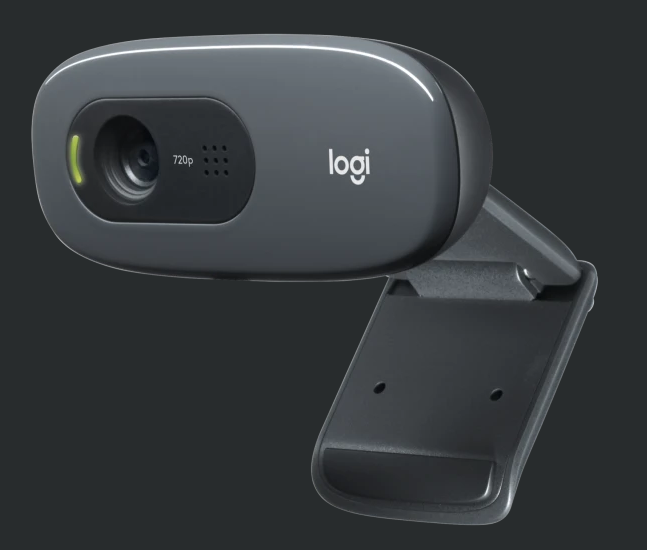
\includegraphics[width=0.7\linewidth]{Images/logitech.png}
	\caption{Logitech Camera}
\end{figure}


\section{The Jetson Nano and the Competition}

System-on-a-Chip (SoC) platforms offer a cost-effective solution for developing low-power, autonomous deep-learning applications, particularly focusing on inference tasks where pre-trained machine learning models are applied to real-world data. Among these, the NVIDIA Jetson Nano stands out as the smallest AI module in the Jetson family, delivering high processing performance with moderate energy requirements. Designed to meet the growing demand for machine learning applications in embedded systems, the Jetson Nano provides a compact and efficient solution. The increasing availability of affordable SoC systems in the lower price range has further democratized access to such technology. These systems incorporate specialized computational kernels, enabling efficient execution of AI workloads while maintaining low power consumption, making them ideal for developers and innovators in edge computing and AI integration. \cite{NVI2024}

Intel offers an affordable solution for developers with the Neural Compute Stick, a compact device designed to easily integrate with existing hardware like Raspberry Pi via a USB connection. Priced at approximately €70, this device features 16 cores powered by the Movidius Myriad X Vision Processing Unit, a low-power processor optimized for image processing tasks. The Neural Compute Stick is compatible with major operating systems, including Windows 10, Ubuntu, and macOS, making it a versatile tool for AI development and deployment in diverse environments. \cite{IntelStickDataSheet:2019}

Google caters to the same audience with its Google Edge TPU Boards, priced at approximately €80. These boards are equipped with a Tensor Processing Unit (TPU), leveraging hardware similar to the technology used in Google Cloud for high-performance AI processing. They are fully compatible with popular development tools such as Jupyter Notebooks and Google Colab, providing a streamlined environment for AI experimentation and deployment. Additionally, the Edge TPU Board doubles as a USB 3.0 dongle, offering flexibility for integration with various systems and workflows.
\cite{Vincent:2018,GoogleTensorFlowModel:2019,GoogleCoral:2019}

Similar advancements can be seen in the latest iterations of consumer technology. Apple’s A12 Bionic chip, featured in recent iPhone models, is equipped with 8 cores and can execute up to 5 trillion operations per second, showcasing exceptional computational power for AI tasks. Meanwhile, Samsung’s Exynos 980 integrates a Neural Processing Unit (NPU) for efficient AI processing, and Huawei’s Kirin 990 takes it a step further by incorporating two NPUs, enabling enhanced parallel AI performance. \cite{SamsungExynos980:2020,HuaweiKirin990:2020}

\section{Applications of the Jetson Nano}

The NVIDIA Jetson Nano offers a wide range of applications, from basic tasks commonly associated with devices like the Raspberry Pi to more complex use cases. It functions as a compact yet powerful computer for conventional purposes such as hosting web servers, browsing the internet, document editing, and even serving as an affordable gaming platform. \cite{Kurniawan:2021}

The true strength of the Jetson Nano lies in its seamless integration with artificial intelligence, enabled by the NVIDIA TensorRT software development kit. This toolkit supports high-performance deep learning inference, allowing pre-trained neural networks to be implemented and fine-tuned for specific applications as they adapt to new data. The Jetson Nano thus bridges the gap between general-purpose computing and AI-driven innovation.

A wide array of Jetson-powered projects, shared by the community on NVIDIA’s   \cite{JetsonProjects:2020} , demonstrates its potential. Beyond teleoperation, the Jetson Nano facilitates advanced applications such as collision avoidance, object tracking, and the development of small autonomous vehicles. Its utility extends into industrial domains as well. For instance, an Adaptive Traffic Control System leverages real-time visual traffic analysis to optimize signal timings and reduce congestion. Another notable project supports individuals with visual or reading impairments by converting recognized text—both printed and handwritten—into synthesized speech, using only a Jetson Nano and a Pi camera. These applications often employ TensorFlow 2.0 and Google Colab for model training.

Additionally, the Jetson Nano, in combination with pre-trained AI models, can be used for a variety of recognition tasks, including sign language interpretation, facial recognition, and object detection. These capabilities highlight the device’s versatility, making it an invaluable tool for both hobbyists and professionals in AI and embedded systems.

\subsection{Processing Power}


The Jetson Nano boasts 472 GFLOPs of processing power, making it highly capable of running modern Artificial Intelligence (AI) algorithms efficiently. It supports the simultaneous operation of multiple neural networks and can process data from numerous high-resolution sensors, making it ideal for use in Network Video Recorders (NVRs) and intelligent gateways. The system is powered by an NVIDIA Maxwell™ architecture GPU with 128 NVIDIA CUDA® cores, capable of delivering up to 0.5 TFLOPs of performance (FP16). Additionally, it features a Quad-core ARM® Cortex®-A57 MPCore processor. With 4 GB of 64-bit LPDDR4 RAM running at 1600 MHz (offering a bandwidth of 25.6 GB/s) and 16 GB of eMMC 5.1 Flash storage, the Jetson Nano provides robust multitasking performance and ample storage for various AI-driven tasks.

\subsection{Connectivity}

The Jetson Nano supports WiFi connectivity through an add-on chip, allowing it to connect via 802.11b/g/n. Alternatively, an Ethernet cable can be used for network access, with speed varying depending on the type of cable (10/100/1000 BASE-T).

\subsection{Data Quality}

\subsection*{Input Data Resolution}
\begin{itemize}[leftmargin=1.5cm]
	\item The system relies on high-resolution image data from sensors like the Logitech C270 HD Webcam, which supports 720p video.
	\item Ensuring that input images are clear, well-lit, and free from motion blur is essential for accurate AI processing.
\end{itemize}

\subsection*{Sensor Accuracy}
\begin{itemize}[leftmargin=1.5cm]
	\item The camera and other connected sensors must be calibrated for precise data capture.
	\item Poor calibration can result in distorted images or erroneous data, affecting AI inference accuracy.
\end{itemize}

\subsection*{Noise and Signal Integrity}
\begin{itemize}[leftmargin=1.5cm]
	\item Image data should have minimal noise to ensure reliable detection and recognition.
	\item Environmental factors such as low light, glare, or reflections can degrade data quality and require preprocessing or enhancement techniques.
\end{itemize}

\subsection*{Consistency in Data Capture}
\begin{itemize}[leftmargin=1.5cm]
	\item To maintain uniformity in AI performance, data must be consistently captured under similar conditions (e.g., resolution, frame rate, angle).
	\item Variability in data input can reduce model accuracy.
\end{itemize}

\subsection*{Data Preparation for AI Models}
\begin{itemize}[leftmargin=1.5cm]
	\item Before feeding data into AI algorithms, preprocessing steps like resizing, normalization, and augmentation (e.g., flipping, rotation) should be applied to improve the robustness of the model.
\end{itemize}

\subsection*{Real-Time Processing Requirements}
\begin{itemize}[leftmargin=1.5cm]
	\item For applications such as license plate recognition, the Jetson Nano must process incoming data in real-time.
	\item Ensuring low-latency data transmission from sensors and efficient handling by the system is key to maintaining quality.
\end{itemize}

\subsection{Data Quantity}

\subsection*{Training Data Requirements}
\begin{itemize}[leftmargin=1.5cm]
	\item To effectively train machine learning models on the Jetson Nano, datasets must include thousands of diverse examples. For instance:
	\begin{itemize}
		\item \textbf{License Plate Recognition:} Datasets should have thousands of images representing different fonts, plate designs, angles, and lighting conditions.
		\item \textbf{Object Detection:} Large datasets, such as COCO or custom datasets, are necessary to ensure model robustness and accuracy.
	\end{itemize}
\end{itemize}

\subsection*{Real-Time Data Handling}
\begin{itemize}[leftmargin=1.5cm]
	\item The Jetson Nano processes real-time data from connected sensors. For a camera streaming at 30 frames per second (fps) in 720p resolution:
	\begin{itemize}
		\item Each frame is approximately 1 MB, leading to a data throughput of ~30 MB/s.
		\item This requires efficient processing to ensure no frame is dropped.
	\end{itemize}
\end{itemize}

\subsection*{Model Size Considerations}
\begin{itemize}[leftmargin=1.5cm]
	\item Models used for inference on the Jetson Nano need to be optimized for the board’s memory limitations.
	\item Pre-trained models, such as YOLO or SSD, typically range from 50 MB to several hundred MB and should be quantized or pruned to fit within 4 GB RAM constraints.
\end{itemize}

\subsection*{Storage for Collected Data}
\begin{itemize}[leftmargin=1.5cm]
	\item For storing training data, processed outputs, and model weights, the onboard 16 GB eMMC is limited.
	\item External storage, such as an SD card or USB drive, is necessary for larger datasets.
\end{itemize}

\subsection*{Balance of Volume and Quality}
\begin{itemize}[leftmargin=1.5cm]
	\item While large datasets improve generalizability, the focus should remain on high-quality, annotated data to maximize model accuracy with minimal computational overhead.
\end{itemize}

\subsection{Data Types}

\subsection*{Image Data}
\begin{itemize}[leftmargin=1.5cm]
	\item Primary data type processed by the Jetson Nano for applications like object detection, license plate recognition, and facial recognition.
	\item Images are typically captured in formats such as JPEG or PNG from connected cameras (e.g., Logitech C270 HD Webcam).
\end{itemize}

\subsection*{Video Data}
\begin{itemize}[leftmargin=1.5cm]
	\item Streams from connected cameras or pre-recorded files, usually in MP4 or AVI format.
	\item Video is processed frame-by-frame for real-time applications like surveillance or autonomous vehicles.
\end{itemize}

\subsection*{Text Data}
\begin{itemize}[leftmargin=1.5cm]
	\item Extracted from images or video frames via Optical Character Recognition (OCR) tools.
	\item Examples include license plate numbers or other textual information embedded in visual data.
\end{itemize}

\subsection*{Sensor Data}
\begin{itemize}[leftmargin=1.5cm]
	\item Data from peripheral sensors connected via GPIO, I2C, or SPI interfaces.
	\item This may include motion, temperature, or proximity sensor data for multi-modal AI applications.
\end{itemize}

\subsection*{Model Data}
\begin{itemize}[leftmargin=1.5cm]
	\item Pre-trained or custom-trained machine learning models used for inference.
	\item These are typically in formats like ONNX, TensorFlow SavedModel, or PyTorch PT files.
\end{itemize}

\subsection*{Annotation Data}
\begin{itemize}[leftmargin=1.5cm]
	\item Structured data for supervised learning tasks, often stored in JSON or XML format, containing bounding boxes, labels, and other metadata.
\end{itemize}

\subsection{Data Structures}

\subsection*{Image Arrays}
Images are stored as NumPy arrays or TensorFlow/PyTorch tensors representing pixel values. For instance:
\begin{itemize}
	\item \textbf{Grayscale images:} 2D arrays with pixel intensity values.
	\item \textbf{Color images:} 3D arrays with RGB values for each pixel.
\end{itemize}

\textbf{Example:}
\begin{lstlisting}[style=python]
	image = np.array([[255, 128, 0], [255, 0, 255]], dtype=np.uint8)  # RGB image
\end{lstlisting}

\subsection*{Bounding Box Coordinates}
For object detection tasks (e.g., license plate detection), bounding boxes are represented as tuples or lists containing the coordinates $(xmin, ymin, xmax, ymax)$ of the detected object.

\textbf{Example:}
\begin{lstlisting}[style=python]
	bbox = (50, 60, 200, 150)  # Bounding box for license plate
\end{lstlisting}

\subsection*{Labels and Annotations}
Annotations for images are stored in JSON or XML format. These typically include bounding boxes, object labels, and metadata.

\textbf{Example (JSON):}
\begin{lstlisting}[style=json]
	{
		"image": "car_image.jpg",
		"annotations": [{"label": "license_plate", "bbox": [50, 60, 200, 150]}]
	}
\end{lstlisting}

\subsection*{Model Weights and Parameters}
The trained models (e.g., neural networks) are typically represented as weights and biases stored in files like HDF5 or TorchScript. These files contain the parameters required for inference.

\textbf{Example:}
\begin{lstlisting}[style=python]
	model_weights = torch.load('model_weights.pth')
\end{lstlisting}

\subsection*{Sensor Data}
Data from connected sensors (e.g., temperature, motion, or proximity sensors) is often stored in lists or dataframes. These structures store time-series data for real-time processing.

\textbf{Example:}
\begin{lstlisting}[style=python]
	sensor_data = {'time': [1, 2, 3], 'temperature': [22.5, 23.0, 23.5]}
\end{lstlisting}


\section{NVIDIA Jetson Nano Developer Kit}

The NVIDIA Jetson Nano is a Single-Board Computer (SBC) specifically designed for running machine learning algorithms. It provides direct access to its components, inputs, and outputs, making it highly versatile for embedded applications. However, to ensure the protection and longevity of the device, it is recommended to place the board in an appropriate enclosure. Like the Raspberry Pi, the Jetson Nano exposes all its components and connectors, making it easy to use but also susceptible to damage. While the included packaging can be used to assemble the Nano, a dedicated case is advised for better protection. An illustration in the book (Figure 5.1) shows the proper orientation of the Jetson Nano, which is important to note, particularly for understanding the arrangement of digital inputs and outputs.



\section{Construction of the Jetson Nano}


The Jetson Nano board measures approximately 70 × 45 mm when not enclosed in a case. A significant heat sink is attached to the board to help dissipate heat during operation. Beneath the heat sink, the powerful NVIDIA Tegra X1 microchip is located, containing four ARM application processor cores and 128 graphics processing units (GPUs). One illustration in the book shows a top view of the Jetson Nano, highlighting its various interfaces, while another provides a side view, showcasing the board's sockets and connectors.



\subsection{External power supply}

The Jetson Nano requires an external power supply, specifically a 5V DC, 2A power source. This can be connected either through the 5V DC interface or the Micro USB interface. When using the 5V DC interface, a jumper must be used to connect the two pins of J48, located between the camera and power supply connector. The connector has a 2.1mm diameter, with the center pin representing the positive pole. If opting for the Micro USB interface, the jumper should be removed to avoid any interference with the power supply connection.


\subsection{HDMI and display port}

While not essential for all applications, a monitor is extremely useful during setup and for certain tasks. You can connect an external monitor through either the HDMI or DisplayPort interface, both of which support various resolutions, including up to 4K. It is important to note that HDMI-to-DVI adapters are incompatible, so you should use a monitor that supports either native HDMI or DisplayPort. Supported image resolutions are listed in the accompanying table. If a monitor is not required for the application, this should be considered when installing the operating system.


\begin{table}
	\centering
	\begin{tabular}{cc}
		\textbf{Video Encode}  & \textbf{250MP/sec} \\   \hline
		H.264/H.265           & 1 $\times$  4K mit  30 f/sec \\
		H.264/H.265	       & 2 $\times$ 1080p mit 60 f/sec \\
		H.264/H.265	       & 4 $\times$ 1080p mit 30 f/sec \\
		H.264/H.265	       & 4 $\times$ 720p mit 60 f/sec  \\
		H.264/H.265	       & 9 $\times$ 720p mit 30 f/sec \\
	\end{tabular}
	\caption{Supported video encoding formats}\label{Jetson:Aufloesungen}
\end{table}

\subsection{$\mu$USB interface}

An alternative power source can be connected via the µUSB interface, using a 5V 2A power supply. This interface is chosen for its accessibility and availability of affordable power supplies. The Jetson Nano typically consumes between 5W to 10W, so it’s essential to choose a quality power supply. Using a low-quality or incompatible power supply can prevent the Jetson Nano from starting. To minimize voltage drops, a power supply with a shorter cable is recommended.


\subsection{USB 3.0 interfaces}

The Jetson Nano has four USB 3.0 ports. Each port has a maximum current limit of 100mA. If a connected device requires more power, an additional external power source is needed. Devices such as keyboards and mice can be connected directly, as they generally do not exceed this current limit.


\subsection{Ethernet interface}

The Jetson Nano includes an RJ45 Ethernet interface for internet connectivity or network communication. It supports Gigabit Ethernet (10/100/1000BASE-T) and can be connected to a router via a patch cable. Alternatively, a Wi-Fi connection can be established using an optional USB wireless LAN (WLAN) dongle.


\subsection{Status LED}

The status LED on the Jetson Nano indicates the power status. It will flash if the power supply is either too low or too high, signaling potential power issues.


\subsection{GPIOs}

The Jetson Nano features a 40-pin General Purpose Input/Output (GPIO) interface, known as the J41 connector. These pins allow you to connect custom circuits and expand the board’s functionality, enabling the use of components like LEDs or motors. Additionally, the Jetson Nano offers interfaces such as SPI, I2C, and I2S, providing further application possibilities.


\subsection{CSI Camera Connection}

The Jetson Nano has a CSI connector for camera modules, compliant with the MIPI CSI-2 D-PHY 1.1 standard. This connector supports 12 lanes in configurations of 3x4 or 4x2, with data transfer speeds of 1.5 Gb/s per lane. With compatible software, the Jetson Nano can be utilized for image recognition and other camera-based applications.

\subsection{microSD card}


As the Jetson Nano does not have an onboard hard drive, it uses a microSD card for storage, including the operating system and application programs. Selecting an appropriate microSD card is crucial for performance, with a minimum recommendation of a 16GB UHS-1 card. The card slot is located on the underside of the board.

\subsection{Specifications of Jetson Nano}
The specifications of the NVIDIA Jetson Nano is as given in the table below:\\
\begin{table}
	\begin{tabular}{||m{5cm}|m{10cm}||}
		\hline
		\textbf{Item} & \textbf{Specification}\\
		\hline
		GPU & NVIDIA Maxwell architecture with 128 NVIDIA CUDA® cores\\
		\hline
		CPU & Quad-core ARM Cortex-A57 MPCore processor\\
		\hline
		Memory & 4 GB 64-bit LPDDR4, 1600MHz 25.6 GB/s\\
		\hline
		Storage & 16 GB eMMC 5.1\\
		\hline
		Video encode & 250MP/sec
		1x 4K @ 30 (HEVC)
		2x 1080p @ 60 (HEVC)
		4x 1080p @ 30 (HEVC)
		4x 720p @ 60 (HEVC)
		9x 720p @ 30 (HEVC)\\
		\hline
		Video decode & 500MP/sec
		1x 4K @ 60 (HEVC)
		2x 4K @ 30 (HEVC)
		4x 1080p @ 60 (HEVC)
		8x 1080p @ 30 (HEVC)
		9x 720p @ 60 (HEVC)\\
		\hline
		Camera & 12 lanes (3x4 or 4x2) MIPI CSI-2 D-PHY 1.1 (1.5 Gb/s per pair)\\
		\hline
		Connectivity & Gigabit Ethernet, M.2 Key E\\
		\hline
		Display & HDMI 2.0 and eDP 1.4\\
		\hline
		USB & 4x USB 3.0, USB 2.0 Micro-B\\
		\hline
		Others & GPIO, I2C, I2S, SPI, UART\\
		\hline
		Mechanical & 69.6 mm x 45 mm
		260-pin edge connector\\
		\hline
	\end{tabular}
	\caption{\label{tab:NVIDIA Jetson Nano Specification} NVIDIA Jetson Nano General Specification}
\end{table}

{
	
	\begin{figure}
		\begin{tikzpicture}
			% Platine
			\draw[greenblue,fill=greenblue] (0,0) -- (12.8,0) -- (12.8,10.1) -- (0,10.1) -- cycle;
			
			% J13 Camera
			\foreach \i in {0,...,14}
			{
				\pgfmathsetmacro{\off}{- 0.1275 * \i}
				\pgfmathsetmacro{\xmin}{0.31};
				\pgfmathsetmacro{\xmax}{0.98};
				\pgfmathsetmacro{\ymin}{6.79};
				\pgfmathsetmacro{\ymax}{6.86};
				\draw[copper,fill=copper] ({\xmin}, {\ymax + \off} ) -- (0.98, {\ymax + \off} ) -- (0.98, {\ymin + \off} ) -- ({\xmin}, {\ymin + \off}) -- cycle;
			}
			\draw[grayleft,fill=grayleft] (0.31,6.65) -- (0.47,6.75) -- (0.47,7.32) -- (0.8,7.32) -- (0.8,4.54) -- (0.47,4.54) -- (0.47, 5.1) -- (0.31,5.2) -- cycle;
			\draw[black,fill=black] (0.67,6.95) -- (0.8,6.95) -- (0.8,4.9) --  (0.67, 4.9) -- cycle;
			
			
			
			% Anschlussprozessor
			\foreach \i in {0,...,46}
			{
				\draw[copper,fill=copper] (1.95 + 0.095 * \i,4.0) -- (1.95+0.095*\i,3.76) -- (2+0.095*\i,3.76) -- (2+0.095*\i,4.0) -- cycle;
			}
			\foreach \i in {0,...,38}
			{
				\draw[copper,fill=copper] (6.67+ 0.095 * \i,4.0) -- (6.67+ 0.095 * \i,3.76) -- (6.72+ 0.095 * \i,3.76) -- (6.72+ 0.095 * \i,4.0) -- cycle;
			}
			\draw[greenenglish,line width=2pt,fill=darkpastelgreen] (1.5,7.0) -- (10.85,7.0) -- (10.85, 3.9) -- (1.5,3.9) -- cycle;
			
			
			\draw[black,fill=black] (1.75,4.7) -- (10.65,4.7) -- (10.65,9.88) -- (1.75,9.88) -- cycle;
			%Kühlkörper
			\draw[fill=grayleft!30!grayright, postaction={path fading=west,  fill=grayleft}] (1.8,8.822) -- (10.6,8.822) -- (10.6,9.83) -- (1.8,9.83) -- cycle;
			\draw[fill=grayleft!30!grayright, postaction={path fading=west,  fill=grayleft}] (1.8,8.773) -- (10.6,8.773) -- (10.6,8.521) -- (1.8,8.521) -- cycle;
			
			\draw[fill=grayleft!30!grayright, postaction={path fading=west,  fill=grayleft}] (1.8,7.464) -- (10.6,7.464) -- (10.6,8.472) -- (1.8,8.472) -- cycle;
			\draw[fill=grayleft!30!grayright, postaction={path fading=west,  fill=grayleft}] (1.8,7.415) -- (10.6,7.415) -- (10.6,7.163) -- (1.8,7.163) -- cycle;
			
			\draw[fill=grayleft!30!grayright, postaction={path fading=west,  fill=grayleft}] (1.8,6.106) -- (10.6,6.106) -- (10.6,7.114) -- (1.8,7.114) -- cycle;
			\draw[fill=grayleft!30!grayright, postaction={path fading=west,  fill=grayleft}] (1.8,6.057) -- (10.6,6.057) -- (10.6,5.805) -- (1.8,5.805) -- cycle;
			
			\draw[fill=grayleft!30!grayright, postaction={path fading=west,  fill=grayleft}] (1.8,4.75) -- (10.6,4.75) -- (10.6,5.756) -- (1.8,5.756) -- cycle;
			
			\draw[fill=grayleft!30!graycircle, postaction={path fading=west,  fill=grayleft},domain=0:360] plot ({4.0+0.252*cos(\x)}, {9.326+0.252*sin(\x)});
			\draw[fill=grayleft!30!graycircle, postaction={path fading=west,  fill=grayleft},domain=0:360] plot ({8.4+0.252*cos(\x)}, {9.326+0.252*sin(\x)});
			
			\draw[fill=grayleft!30!graycircle, postaction={path fading=west,  fill=grayleft},domain=0:360] plot ({4.0+0.252*cos(\x)}, {5.252+0.252*sin(\x)});
			\draw[fill=grayleft!30!graycircle, postaction={path fading=west,  fill=grayleft},domain=0:360] plot ({8.4+0.252*cos(\x)}, {5.252+0.252*sin(\x)});
			
			\pgfmathsetmacro{\xmin}{12.2};
			\pgfmathsetmacro{\xmax}{12.62};
			\pgfmathsetmacro{\ymin}{1.42};
			\pgfmathsetmacro{\ymax}{1.69};
			\draw[darkpastelgreen,fill=greenyellow,
			line width=1.6pt] (\xmin, \ymin) -- (\xmin, \ymax) -- (\xmax,\ymax) -- (\xmax, \ymin) -- cycle;
			
			% J40 Buttons
			\pgfmathsetmacro{\xmin}{0.17};
			\pgfmathsetmacro{\xmax}{0.82};
			\pgfmathsetmacro{\ymin}{7.7};
			\pgfmathsetmacro{\ymax}{9};
			\draw[darkcyan,
			line width=1.6pt] (\xmin, \ymin) -- (\xmin, \ymax) -- (\xmax,\ymax) -- (\xmax, \ymin) -- cycle;
			
			\foreach \j in {0,...,1}
			{
				\foreach \i in {0,...,3}
				{
					\pgfmathsetmacro{\d}{0.05}
					\pgfmathsetmacro{\x}{0.35+0.312*\j};
					\pgfmathsetmacro{\y}{7.87+0.312*\i};
					\draw[yellow,fill=yellow] ({\x-\d}, {\y-\d} ) -- ({\x+\d}, {\y-\d}) -- ({\x+\d}, {\y+\d}) -- ({\x-\d}, {\y+\d}) -- cycle;
				}
			}
			\pgfmathsetmacro{\d}{0.05}
			\pgfmathsetmacro{\x}{0.35+0.312};
			\pgfmathsetmacro{\y}{7.87+0.312*0};
			\draw[yellow,thick,fill=fuchsia] ({\x-\d}, {\y-\d} ) -- ({\x+\d}, {\y-\d}) -- ({\x+\d}, {\y+\d}) -- ({\x-\d}, {\y+\d}) -- cycle;
			
			%J44 Serial
			\pgfmathsetmacro{\xmin}{1.2};
			\pgfmathsetmacro{\xmax}{1.5};
			\pgfmathsetmacro{\ymin}{8.02};
			\pgfmathsetmacro{\ymax}{9.95};
			\draw[darkcyan,
			line width=1.6pt] (\xmin, \ymin) -- (\xmin, \ymax) -- (\xmax,\ymax) -- (\xmax, \ymin) -- cycle;
			
			\foreach \j in {0,...,0}
			{
				\foreach \i in {0,...,5}
				{
					\pgfmathsetmacro{\d}{0.05}
					\pgfmathsetmacro{\x}{1.35+0.312*\j};
					\pgfmathsetmacro{\y}{8.2+0.312*\i};
					\draw[yellow,fill=yellow] ({\x-\d}, {\y-\d} ) -- ({\x+\d}, {\y-\d}) -- ({\x+\d}, {\y+\d}) -- ({\x-\d}, {\y+\d}) -- cycle;
				}
			}
			\pgfmathsetmacro{\d}{0.05}
			\pgfmathsetmacro{\x}{1.35};
			\pgfmathsetmacro{\y}{8.2+0.312*0};
			\draw[yellow,thick,fill=fuchsia] ({\x-\d}, {\y-\d} ) -- ({\x+\d}, {\y-\d}) -- ({\x+\d}, {\y+\d}) -- ({\x-\d}, {\y+\d}) -- cycle;
			
			% J48 DC Jumper
			\pgfmathsetmacro{\xmin}{0.175};
			\pgfmathsetmacro{\xmax}{0.83};
			\pgfmathsetmacro{\ymin}{3.908};
			\pgfmathsetmacro{\ymax}{4.24};
			\draw[darkcyan,
			line width=1.6pt] (\xmin, \ymin) -- (\xmin, \ymax) -- (\xmax,\ymax) -- (\xmax, \ymin) -- cycle;
			
			\foreach \j in {0,...,1}
			{
				\foreach \i in {0,...,0}
				{
					\pgfmathsetmacro{\d}{0.05}
					\pgfmathsetmacro{\x}{0.35+0.312*\j};
					\pgfmathsetmacro{\y}{4.074 +0.312*\i};
					\draw[yellow,fill=yellow] ({\x-\d}, {\y-\d} ) -- ({\x+\d}, {\y-\d}) -- ({\x+\d}, {\y+\d}) -- ({\x-\d}, {\y+\d}) -- cycle;
				}
			}
			
			% J38 PoE
			\pgfmathsetmacro{\xmin}{11.95};
			\pgfmathsetmacro{\xmax}{12.57};
			\pgfmathsetmacro{\ymin}{9.27};
			\pgfmathsetmacro{\ymax}{9.9};
			\draw[darkcyan,
			line width=1.6pt] (\xmin, \ymin) -- (\xmin, \ymax) -- (\xmax,\ymax) -- (\xmax, \ymin) -- cycle;
			
			\foreach \j in {0,...,1}
			{
				\foreach \i in {0,...,1}
				{
					\pgfmathsetmacro{\d}{0.05}
					\pgfmathsetmacro{\x}{12.1+0.312*\j};
					\pgfmathsetmacro{\y}{9.42 +0.312*\i};
					\draw[yellow,fill=yellow] ({\x-\d}, {\y-\d} ) -- ({\x+\d}, {\y-\d}) -- ({\x+\d}, {\y+\d}) -- ({\x-\d}, {\y+\d}) -- cycle;
				}
			}
			
			% J41 Expansion
			\pgfmathsetmacro{\xmin}{11.16};
			\pgfmathsetmacro{\xmax}{11.8};
			\pgfmathsetmacro{\ymin}{2.72};
			\pgfmathsetmacro{\ymax}{9.1};
			\draw[darkcyan,
			line width=1.6pt] (\xmin, \ymin) -- (\xmin, \ymax) -- (\xmax,\ymax) -- (\xmax, \ymin) -- cycle;
			
			\foreach \j in {0,...,1}
			{
				\foreach \i in {0,...,19}
				{
					\pgfmathsetmacro{\d}{0.05}
					\pgfmathsetmacro{\x}{11.325+0.312*\j};
					\pgfmathsetmacro{\y}{2.86 +0.323*\i};
					\draw[blue,fill=yellow] ({\x-\d}, {\y-\d} ) -- ({\x+\d}, {\y-\d}) -- ({\x+\d}, {\y+\d}) -- ({\x-\d}, {\y+\d}) -- cycle;
				}
			}
			\pgfmathsetmacro{\d}{0.05}
			\pgfmathsetmacro{\x}{11.325+0.312};
			\pgfmathsetmacro{\y}{2.86};
			\draw[yellow,thick,fill=fuchsia] ({\x-\d}, {\y-\d} ) -- ({\x+\d}, {\y-\d}) -- ({\x+\d}, {\y+\d}) -- ({\x-\d}, {\y+\d}) --    cycle;
			
			% J15 5V Fan
			\pgfmathsetmacro{\xmin}{9.33};
			\pgfmathsetmacro{\xmax}{10.55};
			\pgfmathsetmacro{\ymin}{2.86};
			\pgfmathsetmacro{\ymax}{3.55};
			\draw[darkcyan,
			line width=1.6pt] (\xmin, \ymin) -- (\xmin, \ymax) -- (\xmax,\ymax) -- (\xmax, \ymin) -- cycle;
			
			\pgfmathsetmacro{\xmin}{9.8};
			\pgfmathsetmacro{\xmax}{10.45};
			\pgfmathsetmacro{\ymin}{3.35};
			\pgfmathsetmacro{\ymax}{3.55};
			\draw[darkcyan,
			line width=1.6pt] (\xmin, \ymin) -- (\xmin, \ymax) -- (\xmax,\ymax) -- (\xmax, \ymin) -- cycle;
			
			\foreach \j in {0,...,3}
			{
				\foreach \i in {0,...,0}
				{
					\pgfmathsetmacro{\d}{0.05}
					\pgfmathsetmacro{\x}{9.45+0.317*\j};
					\pgfmathsetmacro{\y}{3.18 +0.323*\i};
					\draw[blue,fill=yellow] ({\x-\d}, {\y-\d} ) -- ({\x+\d}, {\y-\d}) -- ({\x+\d}, {\y+\d}) -- ({\x-\d}, {\y+\d}) -- cycle;
				}
			}
			
			\pgfmathsetmacro{\d}{0.05}
			\pgfmathsetmacro{\d}{0.05}
			\pgfmathsetmacro{\x}{9.45+0.951};
			\pgfmathsetmacro{\y}{3.18};
			
			\draw[yellow,thick,fill=fuchsia] ({\x-\d}, {\y-\d} ) -- ({\x+\d}, {\y-\d}) -- ({\x+\d}, {\y+\d}) -- ({\x-\d}, {\y+\d}) -- cycle;
			
			
			% Schwarze Flecken
			\pgfmathsetmacro{\xmin}{0.902};
			\pgfmathsetmacro{\xmax}{1.058};
			\pgfmathsetmacro{\ymin}{8.12};
			\pgfmathsetmacro{\ymax}{8.25};
			\draw[black,fill=grayleft!30!grayright, postaction={path fading=west,  fill=grayleft},
			line width=1.0pt] (\xmin, \ymin) -- (\xmin, \ymax) -- (\xmax,\ymax) -- (\xmax, \ymin) -- cycle;
			
			\pgfmathsetmacro{\xmin}{0.902};
			\pgfmathsetmacro{\xmax}{1.058};
			\pgfmathsetmacro{\ymin}{8.74};
			\pgfmathsetmacro{\ymax}{8.87};
			\draw[black,fill=grayleft!30!grayright, postaction={path fading=west,  fill=grayleft},
			line width=1.0pt] (\xmin, \ymin) -- (\xmin, \ymax) -- (\xmax,\ymax) -- (\xmax, \ymin) -- cycle;
			
			\pgfmathsetmacro{\xmin}{0.942};
			\pgfmathsetmacro{\xmax}{1.098};
			\pgfmathsetmacro{\ymin}{7.29};
			\pgfmathsetmacro{\ymax}{7.42};
			\draw[black, fill=grayleft!30!grayright, postaction={path fading=west,  fill=grayleft},
			line width=1.0pt] (\xmin, \ymin) -- (\xmin, \ymax) -- (\xmax,\ymax) -- (\xmax, \ymin) -- cycle;
			
			\pgfmathsetmacro{\xmin}{1.382};
			\pgfmathsetmacro{\xmax}{1.538};
			\pgfmathsetmacro{\ymin}{7.74};
			\pgfmathsetmacro{\ymax}{7.87};
			\draw[black, fill=grayleft!30!grayright, postaction={path fading=west,  fill=grayleft},
			line width=1.0pt] (\xmin, \ymin) -- (\xmin, \ymax) -- (\xmax,\ymax) -- (\xmax, \ymin) -- cycle;
			
			\pgfmathsetmacro{\xmin}{1.35};
			\pgfmathsetmacro{\xmax}{1.49};
			\pgfmathsetmacro{\ymin}{7.2};
			\pgfmathsetmacro{\ymax}{7.37};
			\draw[black, fill=grayleft!30!grayright, postaction={path fading=west,  fill=grayleft},
			line width=1.0pt] (\xmin, \ymin) -- (\xmin, \ymax) -- (\xmax,\ymax) -- (\xmax, \ymin) -- cycle;
			
			\pgfmathsetmacro{\xmin}{1.13};
			\pgfmathsetmacro{\xmax}{1.47};
			\pgfmathsetmacro{\ymin}{3.43};
			\pgfmathsetmacro{\ymax}{3.7};
			\draw[black, fill=grayleft!30!grayright, postaction={path fading=west,  fill=grayleft},
			line width=1.0pt] (\xmin, \ymin) -- (\xmin, \ymax) -- (\xmax,\ymax) -- (\xmax, \ymin) -- cycle;
			
			\pgfmathsetmacro{\xmin}{0.97};
			\pgfmathsetmacro{\xmax}{1.47};
			\pgfmathsetmacro{\ymin}{2.81};
			\pgfmathsetmacro{\ymax}{3.31};
			\draw[black, fill=grayleft!30!grayright, postaction={path fading=west,  fill=grayleft},
			line width=1.0pt] (\xmin, \ymin) -- (\xmin, \ymax) -- (\xmax,\ymax) -- (\xmax, \ymin) -- cycle;
			
			% 5V DC (2.1mm ID, Positive Center)  Stecker
			\pgfmathsetmacro{\xmin}{0.28};
			\pgfmathsetmacro{\xmax}{1.51};
			\pgfmathsetmacro{\ymin}{-0.1};
			\pgfmathsetmacro{\ymax}{1.7};
			\draw[black, fill=black,
			line width=1.0pt] (\xmin, \ymin) -- (\xmin, \ymax) -- (\xmax,\ymax) -- (\xmax, \ymin) -- cycle;
			
			\pgfmathsetmacro{\xmin}{0.32};
			\pgfmathsetmacro{\xmax}{1.47};
			\pgfmathsetmacro{\ymin}{-0.06};
			\pgfmathsetmacro{\ymax}{0.28};
			\draw[black, fill=grayleft!30!grayright, postaction={path fading=west,  fill=grayleft},
			line width=1.0pt] (\xmin, \ymin) -- (\xmin, \ymax) -- (\xmax,\ymax) -- (\xmax, \ymin) -- cycle;
			
			\pgfmathsetmacro{\xmin}{0.32};
			\pgfmathsetmacro{\xmax}{1.47};
			\pgfmathsetmacro{\ymin}{0.32};
			\pgfmathsetmacro{\ymax}{1.65};
			\draw[left color=grayleft, right color=black, middle color=graycircle,
			line width=0pt] (\xmin, \ymin) -- (\xmin, \ymax) -- (\xmax,\ymax) -- (\xmax, \ymin) -- cycle;
			
			
			% Display Port und HDMI
			\pgfmathsetmacro{\xmin}{2.03};
			\pgfmathsetmacro{\xmax}{4.08};
			\pgfmathsetmacro{\ymin}{0};
			\pgfmathsetmacro{\ymax}{2.15};
			\draw[graycircle!50, fill=white!20!graylight, postaction={path fading=west,  fill=grayright!60},
			line width=1.0pt] (\xmin, \ymin) -- (\xmin, \ymax) -- (\xmax,\ymax) -- (\xmax, \ymin) -- cycle;
			
			\draw[greenblue,fill=greenblue] 
			(2.30, 0.7) -- (2.39, 0.22) -- (2.58,0.22) -- (2.68, 0.7) -- 
			(2.52, 0.27) -- (2.46,0.27) -- cycle;
			
			\begin{scope}[xshift=27.3]
				\draw[greenblue,fill=greenblue] 
				(2.30, 0.7) -- (2.39, 0.22) -- (2.58,0.22) -- (2.68, 0.7) -- 
				(2.52, 0.27) -- (2.46,0.27) -- cycle;
			\end{scope}
			
			% USB 3.0 2-mal
			\pgfmathsetmacro{\xmin}{4.6};
			\pgfmathsetmacro{\xmax}{6.31};
			\pgfmathsetmacro{\ymin}{-0.1};
			\pgfmathsetmacro{\ymax}{2.05};
			\draw[graycircle!50, fill=white!20!graylight, postaction={path fading=west,  fill=grayright!60},
			line width=1.0pt] (\xmin, \ymin) -- (\xmin, \ymax) -- (\xmax,\ymax) -- (\xmax, \ymin) -- cycle;
			
			\draw[greenblue,fill=greenblue] 
			(4.83, 0.82) -- (4.93, 0.07) -- (5.14,0.07) -- (5.25, 0.82) -- 
			(5.08, 0.14) -- (5.0,0.14) -- cycle;
			
			\draw[greenblue,fill=greenblue] 
			(5.63, 0.82) -- (5.73, 0.07) -- (5.94,0.07) -- (6.05, 0.82) -- 
			(5.88, 0.14) -- (5.8,0.14) -- cycle;
			
			
			% USB 3.0 2-mal
			\begin{scope}[xshift=63]
				\pgfmathsetmacro{\xmin}{4.6};
				\pgfmathsetmacro{\xmax}{6.31};
				\pgfmathsetmacro{\ymin}{-0.1};
				\pgfmathsetmacro{\ymax}{2.05};
				\draw[graycircle!50, fill=white!20!graylight, postaction={path fading=west,  fill=grayright!60},
				line width=1.0pt] (\xmin, \ymin) -- (\xmin, \ymax) -- (\xmax,\ymax) -- (\xmax, \ymin) -- cycle;
				
				\draw[greenblue,fill=greenblue] 
				(4.83, 0.82) -- (4.93, 0.07) -- (5.14,0.07) -- (5.25, 0.82) -- 
				(5.08, 0.14) -- (5.0,0.14) -- cycle;
				
				\draw[greenblue,fill=greenblue] 
				(5.63, 0.82) -- (5.73, 0.07) -- (5.94,0.07) -- (6.05, 0.82) -- 
				(5.88, 0.14) -- (5.8,0.14) -- cycle;
			\end{scope}
			
			% GigEth
			\pgfmathsetmacro{\xmin}{8.84};
			\pgfmathsetmacro{\xmax}{10.8};
			\pgfmathsetmacro{\ymin}{-0.1};
			\pgfmathsetmacro{\ymax}{2.62};
			\draw[graycircle!50, fill=white!20!graylight, postaction={path fading=west,  fill=grayright!60},
			line width=1.0pt] (\xmin, \ymin) -- (\xmin, \ymax) -- (\xmax,\ymax) -- (\xmax, \ymin) -- cycle;
			
			% Micro USB, PWR oder USB device
			\pgfmathsetmacro{\xmin}{11.285};
			\pgfmathsetmacro{\xmax}{12.225};
			\pgfmathsetmacro{\ymin}{0};
			\pgfmathsetmacro{\ymax}{0.83};
			\draw[graycircle!50, fill=white!20!graylight, postaction={path fading=west,  fill=grayright!60},
			line width=1.0pt] (\xmin, \ymin) -- (\xmin, \ymax) -- (\xmax,\ymax) -- (\xmax, \ymin) -- cycle;
			
			\draw[greenblue,fill=greenblue] 
			(11.41, 0.38) -- (11.475, 0.08) -- (11.585,0.08) -- (11.65, 0.38) -- 
			(11.55, 0.12) -- (11.52,0.12) -- cycle;
			
			\begin{scope}[xshift=12.5]
				\draw[greenblue,fill=greenblue] 
				(11.41, 0.38) -- (11.475, 0.08) -- (11.585,0.08) -- (11.65, 0.38) -- 
				(11.55, 0.12) -- (11.52,0.12) -- cycle;
			\end{scope}
			
		\end{tikzpicture}
		\caption{Jetson Nano: Oversight}\label{JetsonAufsicht}
	\end{figure}

\begin{figure}
	
	\centering		
	\begin{tikzpicture}[scale=0.75]
		% Platine
		\draw[greenblue,fill=greenblue] (0,0) -- (12.8,0) -- (12.8,10.1) -- (0,10.1) -- cycle;
		
		% J13 Camera
		\foreach \i in {0,...,14}
		{
			\pgfmathsetmacro{\off}{- 0.1275 * \i}
			\pgfmathsetmacro{\xmin}{0.31};
			\pgfmathsetmacro{\xmax}{0.98};
			\pgfmathsetmacro{\ymin}{6.79};
			\pgfmathsetmacro{\ymax}{6.86};
			\draw[copper,fill=copper] ({\xmin}, {\ymax + \off} ) -- (0.98, {\ymax + \off} ) -- (0.98, {\ymin + \off} ) -- ({\xmin}, {\ymin + \off}) -- cycle;
		}
		\draw[grayleft,fill=grayleft] (0.31,6.65) -- (0.47,6.75) -- (0.47,7.32) -- (0.8,7.32) -- (0.8,4.54) -- (0.47,4.54) -- (0.47, 5.1) -- (0.31,5.2) -- cycle;
		\draw[black,fill=black] (0.67,6.95) -- (0.8,6.95) -- (0.8,4.9) --  (0.67, 4.9) -- cycle;
		
		\node (J13) at (-1,6) {\begin{tabular}{l} J13\\ Kamera \end{tabular}};
		
		
		% Anschlussprozessor
		\foreach \i in {0,...,46}
		{
			\draw[copper,fill=copper] (1.95 + 0.095 * \i,4.0) -- (1.95+0.095*\i,3.76) -- (2+0.095*\i,3.76) -- (2+0.095*\i,4.0) -- cycle;
		}
		\foreach \i in {0,...,38}
		{
			\draw[copper,fill=copper] (6.67+ 0.095 * \i,4.0) -- (6.67+ 0.095 * \i,3.76) -- (6.72+ 0.095 * \i,3.76) -- (6.72+ 0.095 * \i,4.0) -- cycle;
		}
		\draw[greenenglish,line width=2pt,fill=darkpastelgreen] (1.5,7.0) -- (10.85,7.0) -- (10.85, 3.9) -- (1.5,3.9) -- cycle;
		
		
		\draw[black,fill=black] (1.75,4.7) -- (10.65,4.7) -- (10.65,9.88) -- (1.75,9.88) -- cycle;
		%Kühlkörper
		\draw[fill=grayleft!30!grayright, postaction={path fading=west,  fill=grayleft}] (1.8,8.822) -- (10.6,8.822) -- (10.6,9.83) -- (1.8,9.83) -- cycle;
		\draw[fill=grayleft!30!grayright, postaction={path fading=west,  fill=grayleft}] (1.8,8.773) -- (10.6,8.773) -- (10.6,8.521) -- (1.8,8.521) -- cycle;
		
		\draw[fill=grayleft!30!grayright, postaction={path fading=west,  fill=grayleft}] (1.8,7.464) -- (10.6,7.464) -- (10.6,8.472) -- (1.8,8.472) -- cycle;
		\draw[fill=grayleft!30!grayright, postaction={path fading=west,  fill=grayleft}] (1.8,7.415) -- (10.6,7.415) -- (10.6,7.163) -- (1.8,7.163) -- cycle;
		
		\draw[fill=grayleft!30!grayright, postaction={path fading=west,  fill=grayleft}] (1.8,6.106) -- (10.6,6.106) -- (10.6,7.114) -- (1.8,7.114) -- cycle;
		\draw[fill=grayleft!30!grayright, postaction={path fading=west,  fill=grayleft}] (1.8,6.057) -- (10.6,6.057) -- (10.6,5.805) -- (1.8,5.805) -- cycle;
		
		\draw[fill=grayleft!30!grayright, postaction={path fading=west,  fill=grayleft}] (1.8,4.75) -- (10.6,4.75) -- (10.6,5.756) -- (1.8,5.756) -- cycle;
		
		\draw[fill=grayleft!30!graycircle, postaction={path fading=west,  fill=grayleft},domain=0:360] plot ({4.0+0.252*cos(\x)}, {9.326+0.252*sin(\x)});
		\draw[fill=grayleft!30!graycircle, postaction={path fading=west,  fill=grayleft},domain=0:360] plot ({8.4+0.252*cos(\x)}, {9.326+0.252*sin(\x)});
		
		\draw[fill=grayleft!30!graycircle, postaction={path fading=west,  fill=grayleft},domain=0:360] plot ({4.0+0.252*cos(\x)}, {5.252+0.252*sin(\x)});
		\draw[fill=grayleft!30!graycircle, postaction={path fading=west,  fill=grayleft},domain=0:360] plot ({8.4+0.252*cos(\x)}, {5.252+0.252*sin(\x)});
		
		\pgfmathsetmacro{\xmin}{12.2};
		\pgfmathsetmacro{\xmax}{12.62};
		\pgfmathsetmacro{\ymin}{1.42};
		\pgfmathsetmacro{\ymax}{1.69};
		\draw[darkpastelgreen,fill=greenyellow,
		line width=1.6pt] (\xmin, \ymin) -- (\xmin, \ymax) -- (\xmax,\ymax) -- (\xmax, \ymin) -- cycle;
		
		% J40 Buttons
		\pgfmathsetmacro{\xmin}{0.17};
		\pgfmathsetmacro{\xmax}{0.82};
		\pgfmathsetmacro{\ymin}{7.7};
		\pgfmathsetmacro{\ymax}{9};
		\draw[darkcyan,
		line width=1.6pt] (\xmin, \ymin) -- (\xmin, \ymax) -- (\xmax,\ymax) -- (\xmax, \ymin) -- cycle;
		
		\foreach \j in {0,...,1}
		{
			\foreach \i in {0,...,3}
			{
				\pgfmathsetmacro{\d}{0.05}
				\pgfmathsetmacro{\x}{0.35+0.312*\j};
				\pgfmathsetmacro{\y}{7.87+0.312*\i};
				\draw[yellow,fill=yellow] ({\x-\d}, {\y-\d} ) -- ({\x+\d}, {\y-\d}) -- ({\x+\d}, {\y+\d}) -- ({\x-\d}, {\y+\d}) -- cycle;
			}
		}
		\pgfmathsetmacro{\d}{0.05}
		\pgfmathsetmacro{\x}{0.35+0.312};
		\pgfmathsetmacro{\y}{7.87+0.312*0};
		\draw[yellow,thick,fill=fuchsia] ({\x-\d}, {\y-\d} ) -- ({\x+\d}, {\y-\d}) -- ({\x+\d}, {\y+\d}) -- ({\x-\d}, {\y+\d}) -- cycle;
		
		\node (J40) at (-1,8.5) {\begin{tabular}{l}J40 \\ Buttons\end{tabular}};
		
		
		%J44 Serial
		\pgfmathsetmacro{\xmin}{1.2};
		\pgfmathsetmacro{\xmax}{1.5};
		\pgfmathsetmacro{\ymin}{8.02};
		\pgfmathsetmacro{\ymax}{9.95};
		\draw[darkcyan,
		line width=1.6pt] (\xmin, \ymin) -- (\xmin, \ymax) -- (\xmax,\ymax) -- (\xmax, \ymin) -- cycle;
		
		\foreach \j in {0,...,0}
		{
			\foreach \i in {0,...,5}
			{
				\pgfmathsetmacro{\d}{0.05}
				\pgfmathsetmacro{\x}{1.35+0.312*\j};
				\pgfmathsetmacro{\y}{8.2+0.312*\i};
				\draw[yellow,fill=yellow] ({\x-\d}, {\y-\d} ) -- ({\x+\d}, {\y-\d}) -- ({\x+\d}, {\y+\d}) -- ({\x-\d}, {\y+\d}) -- cycle;
			}
		}
		\pgfmathsetmacro{\d}{0.05}
		\pgfmathsetmacro{\x}{1.35};
		\pgfmathsetmacro{\y}{8.2+0.312*0};
		\draw[yellow,thick,fill=fuchsia] ({\x-\d}, {\y-\d} ) -- ({\x+\d}, {\y-\d}) -- ({\x+\d}, {\y+\d}) -- ({\x-\d}, {\y+\d}) -- cycle;
		
		\node (J13) at (1.8,10.6) {\begin{tabular}{l} J44\\ Serial \end{tabular}};
		
		% J48 DC Jumper
		\pgfmathsetmacro{\xmin}{0.175};
		\pgfmathsetmacro{\xmax}{0.83};
		\pgfmathsetmacro{\ymin}{3.908};
		\pgfmathsetmacro{\ymax}{4.24};
		\draw[darkcyan,
		line width=1.6pt] (\xmin, \ymin) -- (\xmin, \ymax) -- (\xmax,\ymax) -- (\xmax, \ymin) -- cycle;
		
		\foreach \j in {0,...,1}
		{
			\foreach \i in {0,...,0}
			{
				\pgfmathsetmacro{\d}{0.05}
				\pgfmathsetmacro{\x}{0.35+0.312*\j};
				\pgfmathsetmacro{\y}{4.074 +0.312*\i};
				\draw[yellow,fill=yellow] ({\x-\d}, {\y-\d} ) -- ({\x+\d}, {\y-\d}) -- ({\x+\d}, {\y+\d}) -- ({\x-\d}, {\y+\d}) -- cycle;
			}
		}
		\node (J48) at (-1,4) {\begin{tabular}{l}J48 \\ Jumper\end{tabular}};
		
		
		% J38 PoE
		\pgfmathsetmacro{\xmin}{11.95};
		\pgfmathsetmacro{\xmax}{12.57};
		\pgfmathsetmacro{\ymin}{9.27};
		\pgfmathsetmacro{\ymax}{9.9};
		\draw[darkcyan,
		line width=1.6pt] (\xmin, \ymin) -- (\xmin, \ymax) -- (\xmax,\ymax) -- (\xmax, \ymin) -- cycle;
		
		\foreach \j in {0,...,1}
		{
			\foreach \i in {0,...,1}
			{
				\pgfmathsetmacro{\d}{0.05}
				\pgfmathsetmacro{\x}{12.1+0.312*\j};
				\pgfmathsetmacro{\y}{9.42 +0.312*\i};
				\draw[yellow,fill=yellow] ({\x-\d}, {\y-\d} ) -- ({\x+\d}, {\y-\d}) -- ({\x+\d}, {\y+\d}) -- ({\x-\d}, {\y+\d}) -- cycle;
			}
		}
		
		\node[right] (J48) at (13.0,9.5) {\begin{tabular}{l}J38 \\ PoE\end{tabular}};
		
		
		% J41 Expansion
		\pgfmathsetmacro{\xmin}{11.16};
		\pgfmathsetmacro{\xmax}{11.8};
		\pgfmathsetmacro{\ymin}{2.72};
		\pgfmathsetmacro{\ymax}{9.1};
		\draw[darkcyan,
		line width=1.6pt] (\xmin, \ymin) -- (\xmin, \ymax) -- (\xmax,\ymax) -- (\xmax, \ymin) -- cycle;
		
		\foreach \j in {0,...,1}
		{
			\foreach \i in {0,...,19}
			{
				\pgfmathsetmacro{\d}{0.05}
				\pgfmathsetmacro{\x}{11.325+0.312*\j};
				\pgfmathsetmacro{\y}{2.86 +0.323*\i};
				\draw[blue,fill=yellow] ({\x-\d}, {\y-\d} ) -- ({\x+\d}, {\y-\d}) -- ({\x+\d}, {\y+\d}) -- ({\x-\d}, {\y+\d}) -- cycle;
			}
		}
		\pgfmathsetmacro{\d}{0.05}
		\pgfmathsetmacro{\x}{11.325+0.312};
		\pgfmathsetmacro{\y}{2.86};
		\draw[yellow,thick,fill=fuchsia] ({\x-\d}, {\y-\d} ) -- ({\x+\d}, {\y-\d}) -- ({\x+\d}, {\y+\d}) -- ({\x-\d}, {\y+\d}) --    cycle;
		
		\node[right] (J41) at (13,6) {\begin{tabular}{l}J41 \\ Expansion\end{tabular}};
		
		% J15 5V Fan
		\pgfmathsetmacro{\xmin}{9.33};
		\pgfmathsetmacro{\xmax}{10.55};
		\pgfmathsetmacro{\ymin}{2.86};
		\pgfmathsetmacro{\ymax}{3.55};
		\draw[darkcyan,
		line width=1.6pt] (\xmin, \ymin) -- (\xmin, \ymax) -- (\xmax,\ymax) -- (\xmax, \ymin) -- cycle;
		
		\pgfmathsetmacro{\xmin}{9.8};
		\pgfmathsetmacro{\xmax}{10.45};
		\pgfmathsetmacro{\ymin}{3.35};
		\pgfmathsetmacro{\ymax}{3.55};
		\draw[darkcyan,
		line width=1.6pt] (\xmin, \ymin) -- (\xmin, \ymax) -- (\xmax,\ymax) -- (\xmax, \ymin) -- cycle;
		
		\foreach \j in {0,...,3}
		{
			\foreach \i in {0,...,0}
			{
				\pgfmathsetmacro{\d}{0.05}
				\pgfmathsetmacro{\x}{9.45+0.317*\j};
				\pgfmathsetmacro{\y}{3.18 +0.323*\i};
				\draw[blue,fill=yellow] ({\x-\d}, {\y-\d} ) -- ({\x+\d}, {\y-\d}) -- ({\x+\d}, {\y+\d}) -- ({\x-\d}, {\y+\d}) -- cycle;
			}
		}
		
		\node[right] (J15) at (13,3.3) {\begin{tabular}{l}J15 \\ 5V Fan\end{tabular}};
		
		% Schwarze Flecken
		\pgfmathsetmacro{\xmin}{0.902};
		\pgfmathsetmacro{\xmax}{1.058};
		\pgfmathsetmacro{\ymin}{8.12};
		\pgfmathsetmacro{\ymax}{8.25};
		\draw[black,fill=grayleft!30!grayright, postaction={path fading=west,  fill=grayleft},
		line width=1.0pt] (\xmin, \ymin) -- (\xmin, \ymax) -- (\xmax,\ymax) -- (\xmax, \ymin) -- cycle;
		
		\pgfmathsetmacro{\xmin}{0.902};
		\pgfmathsetmacro{\xmax}{1.058};
		\pgfmathsetmacro{\ymin}{8.74};
		\pgfmathsetmacro{\ymax}{8.87};
		\draw[black,fill=grayleft!30!grayright, postaction={path fading=west,  fill=grayleft},
		line width=1.0pt] (\xmin, \ymin) -- (\xmin, \ymax) -- (\xmax,\ymax) -- (\xmax, \ymin) -- cycle;
		
		\pgfmathsetmacro{\xmin}{0.942};
		\pgfmathsetmacro{\xmax}{1.098};
		\pgfmathsetmacro{\ymin}{7.29};
		\pgfmathsetmacro{\ymax}{7.42};
		\draw[black, fill=grayleft!30!grayright, postaction={path fading=west,  fill=grayleft},
		line width=1.0pt] (\xmin, \ymin) -- (\xmin, \ymax) -- (\xmax,\ymax) -- (\xmax, \ymin) -- cycle;
		
		\pgfmathsetmacro{\xmin}{1.382};
		\pgfmathsetmacro{\xmax}{1.538};
		\pgfmathsetmacro{\ymin}{7.74};
		\pgfmathsetmacro{\ymax}{7.87};
		\draw[black, fill=grayleft!30!grayright, postaction={path fading=west,  fill=grayleft},
		line width=1.0pt] (\xmin, \ymin) -- (\xmin, \ymax) -- (\xmax,\ymax) -- (\xmax, \ymin) -- cycle;
		
		\pgfmathsetmacro{\xmin}{1.35};
		\pgfmathsetmacro{\xmax}{1.49};
		\pgfmathsetmacro{\ymin}{7.2};
		\pgfmathsetmacro{\ymax}{7.37};
		\draw[black, fill=grayleft!30!grayright, postaction={path fading=west,  fill=grayleft},
		line width=1.0pt] (\xmin, \ymin) -- (\xmin, \ymax) -- (\xmax,\ymax) -- (\xmax, \ymin) -- cycle;
		
		\pgfmathsetmacro{\xmin}{1.13};
		\pgfmathsetmacro{\xmax}{1.47};
		\pgfmathsetmacro{\ymin}{3.43};
		\pgfmathsetmacro{\ymax}{3.7};
		\draw[black, fill=grayleft!30!grayright, postaction={path fading=west,  fill=grayleft},
		line width=1.0pt] (\xmin, \ymin) -- (\xmin, \ymax) -- (\xmax,\ymax) -- (\xmax, \ymin) -- cycle;
		
		\pgfmathsetmacro{\xmin}{0.97};
		\pgfmathsetmacro{\xmax}{1.47};
		\pgfmathsetmacro{\ymin}{2.81};
		\pgfmathsetmacro{\ymax}{3.31};
		\draw[black, fill=grayleft!30!grayright, postaction={path fading=west,  fill=grayleft},
		line width=1.0pt] (\xmin, \ymin) -- (\xmin, \ymax) -- (\xmax,\ymax) -- (\xmax, \ymin) -- cycle;
		
		% 5V DC (2.1mm ID, Positive Center)  Stecker
		\pgfmathsetmacro{\xmin}{0.28};
		\pgfmathsetmacro{\xmax}{1.51};
		\pgfmathsetmacro{\ymin}{-0.1};
		\pgfmathsetmacro{\ymax}{1.7};
		\draw[black, fill=black,
		line width=1.0pt] (\xmin, \ymin) -- (\xmin, \ymax) -- (\xmax,\ymax) -- (\xmax, \ymin) -- cycle;
		
		\pgfmathsetmacro{\xmin}{0.32};
		\pgfmathsetmacro{\xmax}{1.47};
		\pgfmathsetmacro{\ymin}{-0.06};
		\pgfmathsetmacro{\ymax}{0.28};
		\draw[black, fill=grayleft!30!grayright, postaction={path fading=west,  fill=grayleft},
		line width=1.0pt] (\xmin, \ymin) -- (\xmin, \ymax) -- (\xmax,\ymax) -- (\xmax, \ymin) -- cycle;
		
		\pgfmathsetmacro{\xmin}{0.32};
		\pgfmathsetmacro{\xmax}{1.47};
		\pgfmathsetmacro{\ymin}{0.32};
		\pgfmathsetmacro{\ymax}{1.65};
		\draw[left color=grayleft, right color=black, middle color=graycircle,
		line width=0pt] (\xmin, \ymin) -- (\xmin, \ymax) -- (\xmax,\ymax) -- (\xmax, \ymin) -- cycle;
		
		
		% Display Port und HDMI
		\pgfmathsetmacro{\xmin}{2.03};
		\pgfmathsetmacro{\xmax}{4.08};
		\pgfmathsetmacro{\ymin}{0};
		\pgfmathsetmacro{\ymax}{2.15};
		\draw[graycircle!50, fill=white!20!graylight, postaction={path fading=west,  fill=grayright!60},
		line width=1.0pt] (\xmin, \ymin) -- (\xmin, \ymax) -- (\xmax,\ymax) -- (\xmax, \ymin) -- cycle;
		
		\draw[greenblue,fill=greenblue] 
		(2.30, 0.7) -- (2.39, 0.22) -- (2.58,0.22) -- (2.68, 0.7) -- 
		(2.52, 0.27) -- (2.46,0.27) -- cycle;
		
		\begin{scope}[xshift=27.3]
			\draw[greenblue,fill=greenblue] 
			(2.30, 0.7) -- (2.39, 0.22) -- (2.58,0.22) -- (2.68, 0.7) -- 
			(2.52, 0.27) -- (2.46,0.27) -- cycle;
		\end{scope}
		
		% USB 3.0 2-mal
		\pgfmathsetmacro{\xmin}{4.6};
		\pgfmathsetmacro{\xmax}{6.31};
		\pgfmathsetmacro{\ymin}{-0.1};
		\pgfmathsetmacro{\ymax}{2.05};
		\draw[graycircle!50, fill=white!20!graylight, postaction={path fading=west,  fill=grayright!60},
		line width=1.0pt] (\xmin, \ymin) -- (\xmin, \ymax) -- (\xmax,\ymax) -- (\xmax, \ymin) -- cycle;
		
		\draw[greenblue,fill=greenblue] 
		(4.83, 0.82) -- (4.93, 0.07) -- (5.14,0.07) -- (5.25, 0.82) -- 
		(5.08, 0.14) -- (5.0,0.14) -- cycle;
		
		\draw[greenblue,fill=greenblue] 
		(5.63, 0.82) -- (5.73, 0.07) -- (5.94,0.07) -- (6.05, 0.82) -- 
		(5.88, 0.14) -- (5.8,0.14) -- cycle;
		
		
		% USB 3.0 2-mal
		\begin{scope}[xshift=63]
			\pgfmathsetmacro{\xmin}{4.6};
			\pgfmathsetmacro{\xmax}{6.31};
			\pgfmathsetmacro{\ymin}{-0.1};
			\pgfmathsetmacro{\ymax}{2.05};
			\draw[graycircle!50, fill=white!20!graylight, postaction={path fading=west,  fill=grayright!60},
			line width=1.0pt] (\xmin, \ymin) -- (\xmin, \ymax) -- (\xmax,\ymax) -- (\xmax, \ymin) -- cycle;
			
			\draw[greenblue,fill=greenblue] 
			(4.83, 0.82) -- (4.93, 0.07) -- (5.14,0.07) -- (5.25, 0.82) -- 
			(5.08, 0.14) -- (5.0,0.14) -- cycle;
			
			\draw[greenblue,fill=greenblue] 
			(5.63, 0.82) -- (5.73, 0.07) -- (5.94,0.07) -- (6.05, 0.82) -- 
			(5.88, 0.14) -- (5.8,0.14) -- cycle;
		\end{scope}
		
		% GigEth
		\pgfmathsetmacro{\xmin}{8.84};
		\pgfmathsetmacro{\xmax}{10.8};
		\pgfmathsetmacro{\ymin}{-0.1};
		\pgfmathsetmacro{\ymax}{2.62};
		\draw[graycircle!50, fill=white!20!graylight, postaction={path fading=west,  fill=grayright!60},
		line width=1.0pt] (\xmin, \ymin) -- (\xmin, \ymax) -- (\xmax,\ymax) -- (\xmax, \ymin) -- cycle;
		
		% Micro USB, PWR oder USB device
		\pgfmathsetmacro{\xmin}{11.285};
		\pgfmathsetmacro{\xmax}{12.225};
		\pgfmathsetmacro{\ymin}{0};
		\pgfmathsetmacro{\ymax}{0.83};
		\draw[graycircle!50, fill=white!20!graylight, postaction={path fading=west,  fill=grayright!60},
		line width=1.0pt] (\xmin, \ymin) -- (\xmin, \ymax) -- (\xmax,\ymax) -- (\xmax, \ymin) -- cycle;
		
		\draw[greenblue,fill=greenblue] 
		(11.41, 0.38) -- (11.475, 0.08) -- (11.585,0.08) -- (11.65, 0.38) -- 
		(11.55, 0.12) -- (11.52,0.12) -- cycle;
		
		\begin{scope}[xshift=12.5]
			\draw[greenblue,fill=greenblue] 
			(11.41, 0.38) -- (11.475, 0.08) -- (11.585,0.08) -- (11.65, 0.38) -- 
			(11.55, 0.12) -- (11.52,0.12) -- cycle;
		\end{scope}
		
		\node[right] (J15) at (13,1.3) {\begin{tabular}{l}PWR \\ LED\end{tabular}};
		
		
	\end{tikzpicture}
	\caption{Jetson Nano: Oversight with labels}\label{JetsonAufsicht}
\end{figure}


\begin{figure}
	
	\begin{tikzpicture}
		% Platine
		\draw[greenblue,fill=greenblue] (0,-0.02) -- (12.35,-0.02) -- (12.35,-0.2) -- (0,-0.2) -- cycle;
		
		% 5V 
		\pgfmathsetmacro{\xmin}{0.2};
		\pgfmathsetmacro{\xmax}{1.4};
		\pgfmathsetmacro{\ymin}{0};
		\pgfmathsetmacro{\ymax}{1.33};
		\draw[black,  fill=grayleft!30!grayright, postaction={path fading=west,  fill=grayleft},  line width=1.0pt] 
		(\xmin, \ymin) -- (\xmin, \ymax) -- (\xmax,\ymax) -- (\xmax, \ymin) -- cycle;
		
		\draw[silver,fill=silver,domain=0:360] plot ({0.8+0.11*cos(\x)}, {0.75+0.11*sin(\x)});
		\draw[silver,fill=silver,domain=230:310] plot ({0.8+0.4*cos(\x)}, {0.75+0.4*sin(\x)});
		\draw[black,line width=1.0pt,domain=0:360] plot ({0.8+0.4*cos(\x)}, {0.75+0.4*sin(\x)});
		
		%Display Port und HDMI
		\pgfmathsetmacro{\xmin}{1.9};
		\pgfmathsetmacro{\xmax}{3.95};
		\pgfmathsetmacro{\ymin}{0};
		\pgfmathsetmacro{\ymax}{2.1};
		\draw[graycircle!50, fill=white!20!graylight, postaction={path fading=west,  fill=grayright!60}, line width=1.0pt
		] (\xmin, \ymin) -- (\xmin, \ymax) -- (\xmax,\ymax) -- (\xmax, \ymin) -- cycle;
		
		\draw[black,fill=grayleft!30!grayright, postaction={path fading=west,  fill=grayleft},
		line width=1.0pt]   (2.4, 0.17) -- (2.17,0.41) -- (2.17,0.64) -- (3.65,0.64) -- (3.65,0.41) -- (3.42,0.17) -- cycle;
		
		\pgfmathsetmacro{\xmin}{2.35};
		\pgfmathsetmacro{\xmax}{3.48};
		\pgfmathsetmacro{\ymin}{0.39};
		\pgfmathsetmacro{\ymax}{0.42};
		\draw[grayright,fill=grayright %graycircle!50, fill=white!20!graylight, postaction={path fading=west,  fill=grayright!60}, line width=1.0pt
		] (\xmin, \ymin) -- (\xmin, \ymax) -- (\xmax,\ymax) -- (\xmax, \ymin) -- cycle;
		
		\draw[black,fill=grayleft!30!grayright, postaction={path fading=west,  fill=grayleft},
		line width=1.0pt] (2.33,1.42) -- (2.1, 1.65) -- (2.1,1.92) -- (3.66,1.92) -- (3.66,1.42) -- cycle;
		\draw[grayright,fill=grayright] (2.47, 1.7) -- (2.47,1.6) -- (2.37, 1.6) -- (2.37,1.75) -- (3.47,1.75) -- (3.47,1.6) -- (3.37,1.6) -- (3.37,1.7) -- cycle;
		
		% USV 3.0 - 2 x 2 
		\foreach \j in {0,...,1}
		{
			\pgfmathsetmacro{\xmin}{4.4+2.15*\j};
			\pgfmathsetmacro{\xmax}{6.1+2.15*\j};
			\pgfmathsetmacro{\ymin}{0};
			\pgfmathsetmacro{\ymax}{1.8};
			\draw[graycircle!50, fill=white!20!graylight, postaction={path fading=west,  fill=grayright!60}, line width=1.0pt] (\xmin, \ymin) -- (\xmin, \ymax) -- (\xmax,\ymax) -- (\xmax, \ymin) -- cycle;
			
			\foreach \i in {0,...,1}
			{
				\pgfmathsetmacro{\xmin}{4.54+2.16*\j};
				\pgfmathsetmacro{\xmax}{5.96+2.16*\j};
				\pgfmathsetmacro{\ymin}{0.27+0.86*\i};
				\pgfmathsetmacro{\ymax}{0.78+0.86*\i};
				\draw[black,fill=grayleft!30!grayright, postaction={path fading=west,  fill=grayleft},
				line width=1.0pt] 
				(\xmin, \ymin) -- (\xmin, \ymax) -- (\xmax,\ymax) -- (\xmax, \ymin) -- cycle;
				
				\pgfmathsetmacro{\xmin}{4.6+2.16*\j};
				\pgfmathsetmacro{\xmax}{5.91+2.16*\j};
				\pgfmathsetmacro{\ymin}{0.52+0.82*\i};
				\pgfmathsetmacro{\ymax}{0.73+0.82*\i};
				\draw[cyan, fill=deepskyblue, line width=1.0pt] 
				(\xmin, \ymin) -- (\xmin, \ymax) -- (\xmax,\ymax) -- (\xmax, \ymin) -- cycle;
				
				\foreach \k in {0,...,3}
				{
					\pgfmathsetmacro{\xmin}{4.75+2.16*\j+0.29*\k};
					\pgfmathsetmacro{\xmax}{4.88+2.16*\j+0.29*\k};
					\pgfmathsetmacro{\ymin}{0.44+0.83*\i};
					\pgfmathsetmacro{\ymax}{0.48+0.83*\i};
					\draw[copper,fill=copper] (\xmin, \ymin) -- (\xmin, \ymax) -- (\xmax,\ymax) -- (\xmax, \ymin) -- cycle;
				}     
			}
		}
		
		% Ethernet
		\pgfmathsetmacro{\xmin}{8.55};
		\pgfmathsetmacro{\xmax}{10.5};
		\pgfmathsetmacro{\ymin}{0};
		\pgfmathsetmacro{\ymax}{1.5};
		\draw[graycircle!50, fill=white!20!graylight, postaction={path fading=west,  fill=grayright!60}, line width=1.0pt] (\xmin, \ymin) -- (\xmin, \ymax) -- (\xmax,\ymax) -- (\xmax, \ymin) -- cycle;
		
		\pgfmathsetmacro{\xmin}{8.8};
		\pgfmathsetmacro{\xmax}{10.2};
		\pgfmathsetmacro{\ymin}{0};
		\pgfmathsetmacro{\ymax}{1.25};
		\draw[black,  fill=grayleft!30!grayright, postaction={path fading=west,  fill=grayleft},  line width=1.0pt] (\xmin, \ymin) -- (\xmin, \ymax) -- (\xmax,\ymax) -- (\xmax, \ymin) -- cycle;
		
		\pgfmathsetmacro{\xmin}{8.8};
		\pgfmathsetmacro{\xmax}{9.25};
		\pgfmathsetmacro{\ymin}{0};
		\pgfmathsetmacro{\ymax}{0.3};
		\draw[darkpastelgreen,fill=greenyellow, line width=1.0pt] (\xmin, \ymin) -- (\xmin, \ymax) -- (\xmax,\ymax) -- (\xmax, \ymin) -- cycle;
		
		\pgfmathsetmacro{\xmin}{9.75};
		\pgfmathsetmacro{\xmax}{10.2};
		\pgfmathsetmacro{\ymin}{0};
		\pgfmathsetmacro{\ymax}{0.3};
		\draw[orange, fill=yellow, line width=1.0pt
		] (\xmin, \ymin) -- (\xmin, \ymax) -- (\xmax,\ymax) -- (\xmax, \ymin) -- cycle;
		
		\foreach \j in {0,...,7}
		{
			\pgfmathsetmacro{\xmin}{9     + 0.13*\j};
			\pgfmathsetmacro{\xmax}{9.068 + 0.13*\j};
			\pgfmathsetmacro{\ymin}{0.92};
			\pgfmathsetmacro{\ymax}{1.25};
			\draw[copper,fill=copper]   (\xmin, \ymin) -- (\xmin, \ymax) -- (\xmax,\ymax) -- (\xmax, \ymin) -- cycle;
		}
		
		\pgfmathsetmacro{\xmin}{11.8};
		\pgfmathsetmacro{\xmax}{12.25};
		\pgfmathsetmacro{\ymin}{0};
		\pgfmathsetmacro{\ymax}{0.1};
		\draw[darkpastelgreen,fill=greenyellow, line width=1.0pt] (\xmin, \ymin) -- (\xmin, \ymax) -- (\xmax,\ymax) -- (\xmax, \ymin) -- cycle;
		
		% HDMI
		\draw[silver,fill=silver, line width=1.0pt] (11.0, 0) -- (11.7,0) -- (11.9,0.17) -- (11.9, 0.35) -- (10.8,0.35) --  (10.8, 0.17) -- cycle;
		
		\draw[black,fill=black] (11.05, 0.125) -- (11.65,0.125) -- (11.75,0.22) -- (11.75, 0.25) -- (10.95,0.25) --  (10.95, 0.22) -- cycle;
		
		\node (P1) at (0.8,-0.6) {5V DC};
		\node (P2) at (3,-0.8) {\begin{tabular}{c} Display Port \\ HDMI \end{tabular}};
		\node (P2) at (5.2,-0.8) {\begin{tabular}{c} USB 3.0 \\ USB 3.0 \end{tabular}};
		\node (P2) at (7.4,-0.8) {\begin{tabular}{c} USB 3.0 \\ USB 3.0 \end{tabular}};
		\node (P2) at (9.5,-0.6) { GigEth };
		\node (P2) at (11.8,-1) {\begin{tabular}{c} Micro USB\\ PWR And \\ USB Device\end{tabular}};
		\node (P2) at (12.9,-1.8) {PWR LED};
		
	\end{tikzpicture}
	\caption{Side view of the Jetson Nano with labels} \label{JetonSeite}
\end{figure}	

}

\section{Jetson Nano Interfaces}
\subsection{J41 Expansion Header Pinout - GPIO Pins}
The Jetson Nano can interface with various external systems, and the ability to control the pins on the J41 header is essential for communication and device management. The pins on the header support several communication protocols:


\begin{itemize}
	\item Universal Asynchronous Receiver Transmitter \ac{uart} for serial communication 
	\item Inter-Integrated Circuit \ac{i2c} for two-wire communication 
	\item Serial Peripheral Interface \ac{spi} for high-speed data transfer
	\item Inter-IC Sound  \ac{i2s} for audio data transmission
	\item General Purpose Input/Output  \ac{gpio} for direct communication
\end{itemize}    

GPIO pins allow for binary signal exchange between systems, functioning as digital inputs and outputs that can be configured as needed. By default, most of the pins on the Jetson Nano are set to GPIO mode, except for pins 3, 5, 8, 9, 27, and 28. Specifically, pins 3 and 5 are used for one of the I2C interfaces (SDA and SCL lines), while pins 27 and 28 serve the second I2C interface. Pins 8 and 10 are designated for the UART's receive (Rx) and transmit (Tx) lines. \cite{JetsonUserManual:2020} 

To utilize the \ac{gpio}, the GPIO library must be installed on the system. \cite{GitHubGPIO:2020}.


\begin{figure}
	\centering
	
	\begin{tikzpicture}[scale=1.4]
		%J44 Serial
		\pgfmathsetmacro{\xmin}{1.2};
		\pgfmathsetmacro{\xmax}{1.5};
		\pgfmathsetmacro{\ymin}{8.02};
		\pgfmathsetmacro{\ymax}{9.95};
		\draw[darkcyan,fill=greenblue,
		line width=1.6pt] (\xmin, \ymin) -- (\xmin, \ymax) -- (\xmax,\ymax) -- (\xmax, \ymin) -- cycle;
		
		\foreach \j in {0,...,0}
		{
			\foreach \i in {0,...,5}
			{
				\pgfmathsetmacro{\d}{0.05}
				\pgfmathsetmacro{\x}{1.35+0.312*\j};
				\pgfmathsetmacro{\y}{8.2+0.312*\i};
				\draw[yellow,fill=yellow] ({\x-\d}, {\y-\d} ) -- ({\x+\d}, {\y-\d}) -- ({\x+\d}, {\y+\d}) -- ({\x-\d}, {\y+\d}) -- cycle;
			}
		}
		\pgfmathsetmacro{\d}{0.05}
		\pgfmathsetmacro{\x}{1.35};
		\pgfmathsetmacro{\y}{8.2+0.312*0};
		\draw[yellow,thick,fill=fuchsia] ({\x-\d}, {\y-\d} ) -- ({\x+\d}, {\y-\d}) -- ({\x+\d}, {\y+\d}) -- ({\x-\d}, {\y+\d}) -- cycle;
		
		\node[right]  (P5) at (1.7,9.81) {CTS};
		\node[right]  (P5) at (1.7,9.48) {TXD};
		\node[right]  (P4) at (1.7,9.16) {TXD};
		\node[right]  (P3) at (1.7,8.82) {N/A};
		\node[right]  (P2) at (1.7,8.51) {RTS};
		\node[right]  (P1) at (1.7,8.16) {GND};
	\end{tikzpicture}
	
	\caption{J44 Serial interface - 3.3V 115200 Baud, 8N1} 
\end{figure}

\begin{figure}
	\centering
	\begin{tikzpicture}[scale=1.4]
		% J40 Buttons
		\pgfmathsetmacro{\xmin}{0.17};
		\pgfmathsetmacro{\xmax}{0.82};
		\pgfmathsetmacro{\ymin}{7.7};
		\pgfmathsetmacro{\ymax}{9};
		\draw[darkcyan,fill=greenblue,
		line width=1.6pt] (\xmin, \ymin) -- (\xmin, \ymax) -- (\xmax,\ymax) -- (\xmax, \ymin) -- cycle;
		
		\foreach \j in {0,...,1}
		{
			\foreach \i in {0,...,3}
			{
				\pgfmathsetmacro{\d}{0.05}
				\pgfmathsetmacro{\x}{0.35+0.312*\j};
				\pgfmathsetmacro{\y}{7.87+0.312*\i};
				\draw[yellow,fill=yellow] ({\x-\d}, {\y-\d} ) -- ({\x+\d}, {\y-\d}) -- ({\x+\d}, {\y+\d}) -- ({\x-\d}, {\y+\d}) -- cycle;
			}
		}
		\pgfmathsetmacro{\d}{0.05}
		\pgfmathsetmacro{\x}{0.35+0.312};
		\pgfmathsetmacro{\y}{7.87+0.312*0};
		\draw[yellow,thick,fill=fuchsia] ({\x-\d}, {\y-\d} ) -- ({\x+\d}, {\y-\d}) -- ({\x+\d}, {\y+\d}) -- ({\x-\d}, {\y+\d}) -- cycle;
		
		\node[right]  (P4) at (1,8.85) {DIS (disable auto power-on)};
		\node[right]  (P3) at (1,8.5) {RST (system reset)};
		\node[right]  (P2) at (1,8.15) {FRC (board recovery mode))};
		\node[right]  (P1) at (1,7.8) {ON (power on) )};
		
	\end{tikzpicture}
	
	\caption{J40 Buttons}
\end{figure}  

\begin{figure}
	\centering
	\begin{tikzpicture}[scale=1.4]
		% J15 5V Fan
		\pgfmathsetmacro{\xmin}{9.33};
		\pgfmathsetmacro{\xmax}{10.55};
		\pgfmathsetmacro{\ymin}{2.86};
		\pgfmathsetmacro{\ymax}{3.55};
		\draw[darkcyan,fill=greenblue,  line width=1.6pt] 
		(\xmin, \ymin) -- (\xmin, \ymax) -- (\xmax,\ymax) -- (\xmax, \ymin) -- cycle;
		
		\pgfmathsetmacro{\xmin}{9.8};
		\pgfmathsetmacro{\xmax}{10.45};
		\pgfmathsetmacro{\ymin}{3.35};
		\pgfmathsetmacro{\ymax}{3.55};
		\draw[darkcyan,
		line width=1.6pt] (\xmin, \ymin) -- (\xmin, \ymax) -- (\xmax,\ymax) -- (\xmax, \ymin) -- cycle;
		
		\foreach \j in {0,...,3}
		{
			\foreach \i in {0,...,0}
			{
				\pgfmathsetmacro{\d}{0.05}
				\pgfmathsetmacro{\x}{9.45+0.317*\j};
				\pgfmathsetmacro{\y}{3.18 +0.323*\i};
				\draw[blue,fill=yellow] ({\x-\d}, {\y-\d} ) -- ({\x+\d}, {\y-\d}) -- ({\x+\d}, {\y+\d}) -- ({\x-\d}, {\y+\d}) -- cycle;
			}
		}
		
		\draw[dotted] (9.45, 3.18) -- (9.45, 4.85) -- (9.6, 4.85);
		\node[right]  (P4) at (9.6,4.85) {PWM};
		\draw[dotted] (9.45+0.317, 3.18) -- (9.45+0.317, 4.5) -- (9.6+0.317, 4.5);
		\node[right]  (P3) at (9.6+0.317,4.5) {Tach};
		\draw[dotted] (9.45+0.317+0.317, 3.18) -- (9.45+0.317+0.317, 4.15) -- (9.6+0.317+0.317, 4.15);
		\node[right]  (P2) at (9.6+0.317+0.317,4.15) {5V};
		\draw[dotted] (9.45+0.317+0.317+0.317, 3.18) -- (9.45+0.317+0.317+0.317, 3.8) -- (9.6+0.317+0.317+0.317, 3.8);
		\node[right]  (P1) at (9.6+0.317+0.317+0.317,3.8) {GND};
		
		\pgfmathsetmacro{\d}{0.05}
		\pgfmathsetmacro{\x}{9.45+0.317*3};
		\pgfmathsetmacro{\y}{3.18};
		\draw[yellow,thick,fill=fuchsia] ({\x-\d}, {\y-\d} ) -- ({\x+\d}, {\y-\d}) -- ({\x+\d}, {\y+\d}) -- ({\x-\d}, {\y+\d}) -- cycle;
		
	\end{tikzpicture}
	
	\caption{J15 5V fan} 
\end{figure}

This section highlights some of the Jetson Nano Developer Kit interfaces.
\begin{itemize}
	\item Module
	\begin{itemize}
		\item [J501] Slot for a microSD card.
		\item The passive heatsink supports up to 10W of power usage for the module at an ambient temperature of 25°C. If additional cooling is required for your application, the module can be configured to control a system fan.
	\end{itemize}
	\item Carrier Board
	\begin{itemize}
		\item (DS3) Power LED; which lights up when the developer kit is powered on.
		\item (J2) SO-DIMM connector for attaching the Jetson Nano module.
		\item (J6] HDMI and DisplayPort (DP) connectors.
		\item (J13) Camera connector for CSI cameras. The Jetson Nano is compatible with IMX219 camera modules, including the Leopard Imaging LI-IMX219-MIPIFF-NANO camera module and the Raspberry Pi Camera Module V2.
		\item (J15) 4-pin fan control header, supporting Pulse Width Modulation (PWM) output and tachometer input.
		\item (J18) M.2 Key E connector, suitable for wireless networking cards. It provides interfaces for PCIe (x1), USB 2.0, UART, I2S, and I2C. To access J18, the Jetson Nano module must be detached.
		\item (J25) Power jack for a 5V 4A power supply, compatible with a 2.1×5.5×9.5 mm plug with positive polarity.
		\item (J28) Micro-USB 2.0 connector, which can serve two purposes: If the J48 pins are not connected, it can power the developer kit with a 5V 2A Micro-USB power supply. If the J48 pins are connected, it operates in Device Mode.
		\item (J32 and J33) Two stacks of USB 3.0 Type-A connectors. Each stack has a total power delivery limit of 1A. All four connectors are linked to the Jetson Nano module through a built-in USB 3.0 hub on the carrier board.
		\item (J38) Power over Ethernet (PoE) header, which passes any DC voltage present on the J43 Ethernet jack, in accordance with IEEE 802.3af standards.
		\item (J40) 8-pin button header, which exposes various system signals related to power, reset, and force recovery.
	\end{itemize}
\end{itemize}

\section{Constraints}

\subsection{Power Supply Constraints}
\begin{itemize}[leftmargin=1.5cm]
	\item Requires a stable 5V, 2A DC power supply for reliable operation.
	\item If using the Micro USB interface for power, the jumper at \texttt{J48} must remain disconnected.
	\item For the 5V DC interface, a jumper is necessary to connect the pins on \texttt{J48}, with proper polarity to avoid damage.
\end{itemize}

\subsection{Environmental Constraints}
\begin{itemize}[leftmargin=1.5cm]
	\item The exposed nature of the board makes it susceptible to physical damage or environmental factors (e.g., dust, humidity). It is recommended to use an enclosure for protection.
\end{itemize}

\subsection{Hardware Limitations}
\begin{itemize}[leftmargin=1.5cm]
	\item Limited onboard storage of 16 GB eMMC 5.1, which may require external storage for large datasets.
	\item RAM is fixed at 4 GB LPDDR4, which could be a bottleneck for highly intensive applications.
\end{itemize}

\subsection{Connectivity Constraints}
\begin{itemize}[leftmargin=1.5cm]
	\item WiFi connectivity is not built-in and requires an add-on module for wireless networking.
	\item Ethernet speed depends on the cable specification (10/100/1000 BASE-T).
\end{itemize}

\subsection{Sensor Input Constraints}
\begin{itemize}[leftmargin=1.5cm]
	\item Limited to supported interfaces like Camera Serial Interface (CSI) and GPIO, which may not be compatible with all sensor types without additional hardware.
\end{itemize}

\subsection{Performance Constraints}
\begin{itemize}[leftmargin=1.5cm]
	\item While capable of handling multiple neural networks, the 472 GFLOPs performance and 4 GB RAM limit scalability for extremely complex models or high-speed real-time processing.
\end{itemize}


\section{Conclusion}

In conclusion, the car license plate detection system powered by the NVIDIA Jetson Nano showcases the potential of edge computing for real-time computer vision tasks. The GPU acceleration of the Jetson Nano enables the efficient execution of deep learning models, making it an ideal choice for processing complex tasks like license plate recognition. With the integration of a high-resolution camera module, the system ensures precise and reliable data capture, contributing to accurate detection performance.

The Jetson Nano's compact form factor and low power consumption make it especially suitable for deployment in environments where space and power are limited. It is well-suited for applications such as surveillance cameras, traffic monitoring, and smart city systems. By providing a cost-effective yet powerful solution, the Jetson Nano is capable of meeting the demands of these resource-constrained scenarios.

Furthermore, by utilizing edge computing, the need for continuous reliance on cloud services is minimized, improving system autonomy and responsiveness. The real-time processing capabilities of the Jetson Nano enable faster decision-making, enhancing the overall efficiency of the license plate detection system. This makes the system a robust and scalable solution for a variety of intelligent transportation and computer vision applications.

